%%%%%%%%%%%%%%%%%%%%%%%%%%%%%%%%%%%%%%%%%%%%%%%%%%%
% PRESENTATION FOR SUMMER RESEARCH MEETING (2018)
% 
% Prithvi Thakur
% Geophysics research group
% Department of Earth and Environmental Science
% University of Michigan, Ann Arbor
%%%%%%%%%%%%%%%%%%%%%%%%%%%%%%%%%%%%%%%%%%%%%%%%%%%

\documentclass{beamer}

\mode<presentation>{
\usetheme{AnnArbor}
}

\usepackage{graphicx} % Allows including images
\usepackage{booktabs} % Allows the use of \toprule, \midrule and \bottomrule in tables
%\usepackage[export]{adjustbox} % To change the default alignment of image
\usepackage{subcaption} % Add subfigures to place figures side by side

%------------------------------------------------
%           TITLE PAGE INFORMATION
%------------------------------------------------
\title[MFD in EQ Cycles]{Magnitude-Frequency Distribution of Simulated Earthquake Cycles in Damaged Fault Zones} 
\author{Prithvi Thakur}
\institute[UofM]
{
University of Michigan \\ % Your institution for the title page
\medskip
\textit{prith@umich.edu} % Your email address
}
\date{\today} % Date, can be changed to a custom date
%------------------------------------------------

%%%%%%%%%%%%%%%%
\begin{document}

% TITLE PAGE
\begin{frame}
    \titlepage 
\end{frame}

% TABLE OF CONTENTS
\begin{frame}
    \frametitle{Overview}
    \begin{itemize}
        \item 2D Numerical simulation of long-term fault slip using a spectral element method. 
        \item Strike-slip fault with mode III rupture (e.g., San Andreas), surrounded by a narrow damaged zone
            of low rigidity (Fault Zone).
        \item Studied the effect of varying fault zone depth on the location of earthquake hypocenter.
        \item Rewrote the matlab code in Julia with some modifications: vectorization, encapsulation of subroutines. The speed is approx. 2.5 times faster than matlab.
    \end{itemize}
\end{frame}

% MODEL DESCRIPTION
\section{Model Description}
\begin{frame}
    \frametitle{Model Description}
    \begin{figure}
        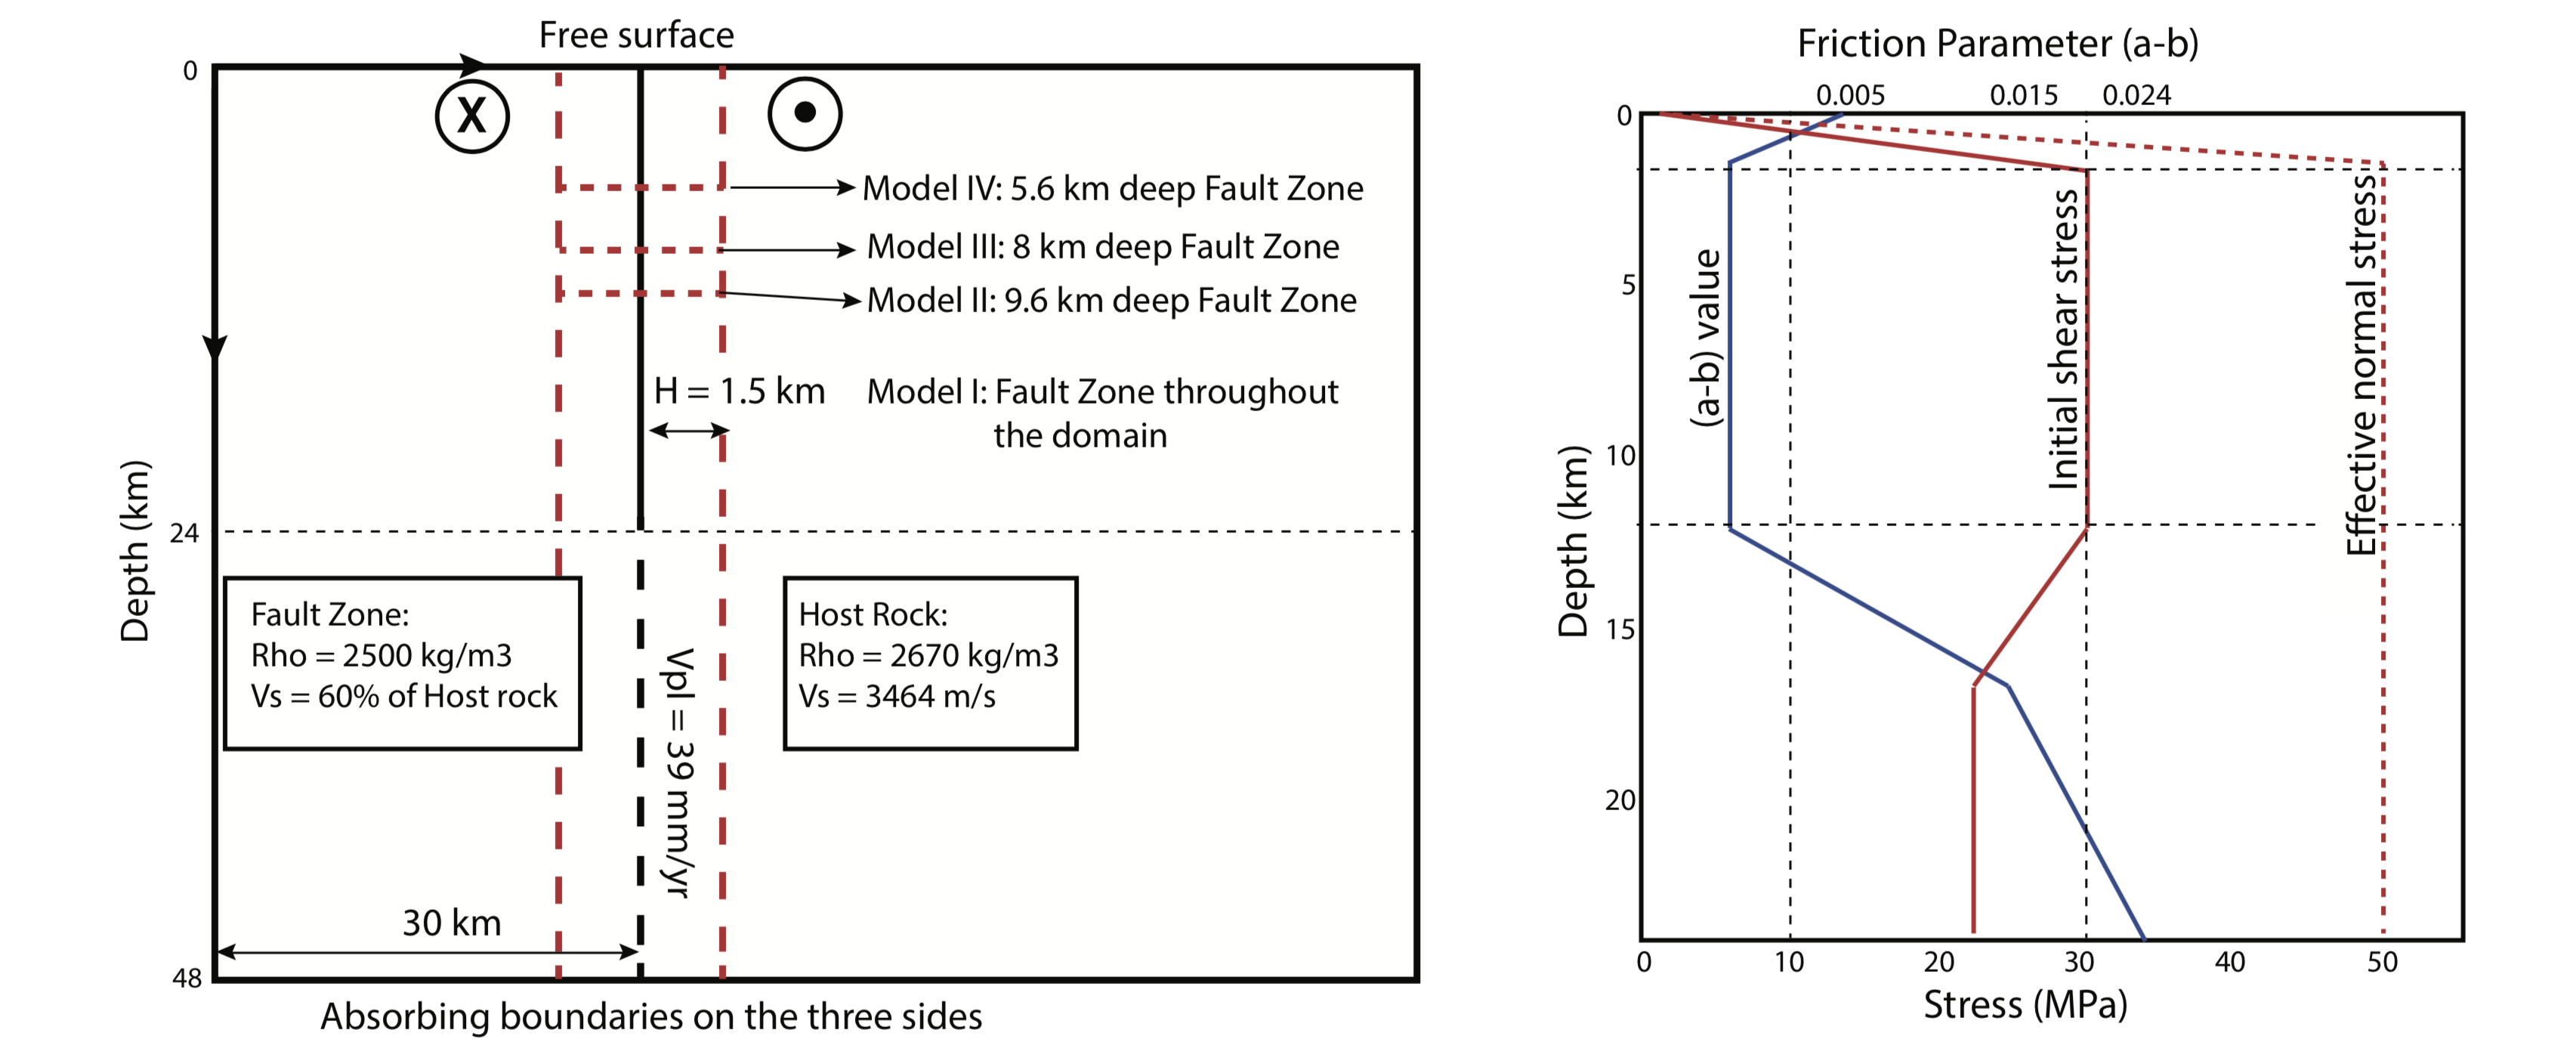
\includegraphics[width=0.9\linewidth]{images/model_setup}
    \end{figure}
\end{frame}

% OBSERVATIONS: PARKFIELD MFD PLOTS
\section{Natural Observations}
\begin{frame}
    \frametitle{Observations from San-Andreas Fault}
    \begin{figure}
        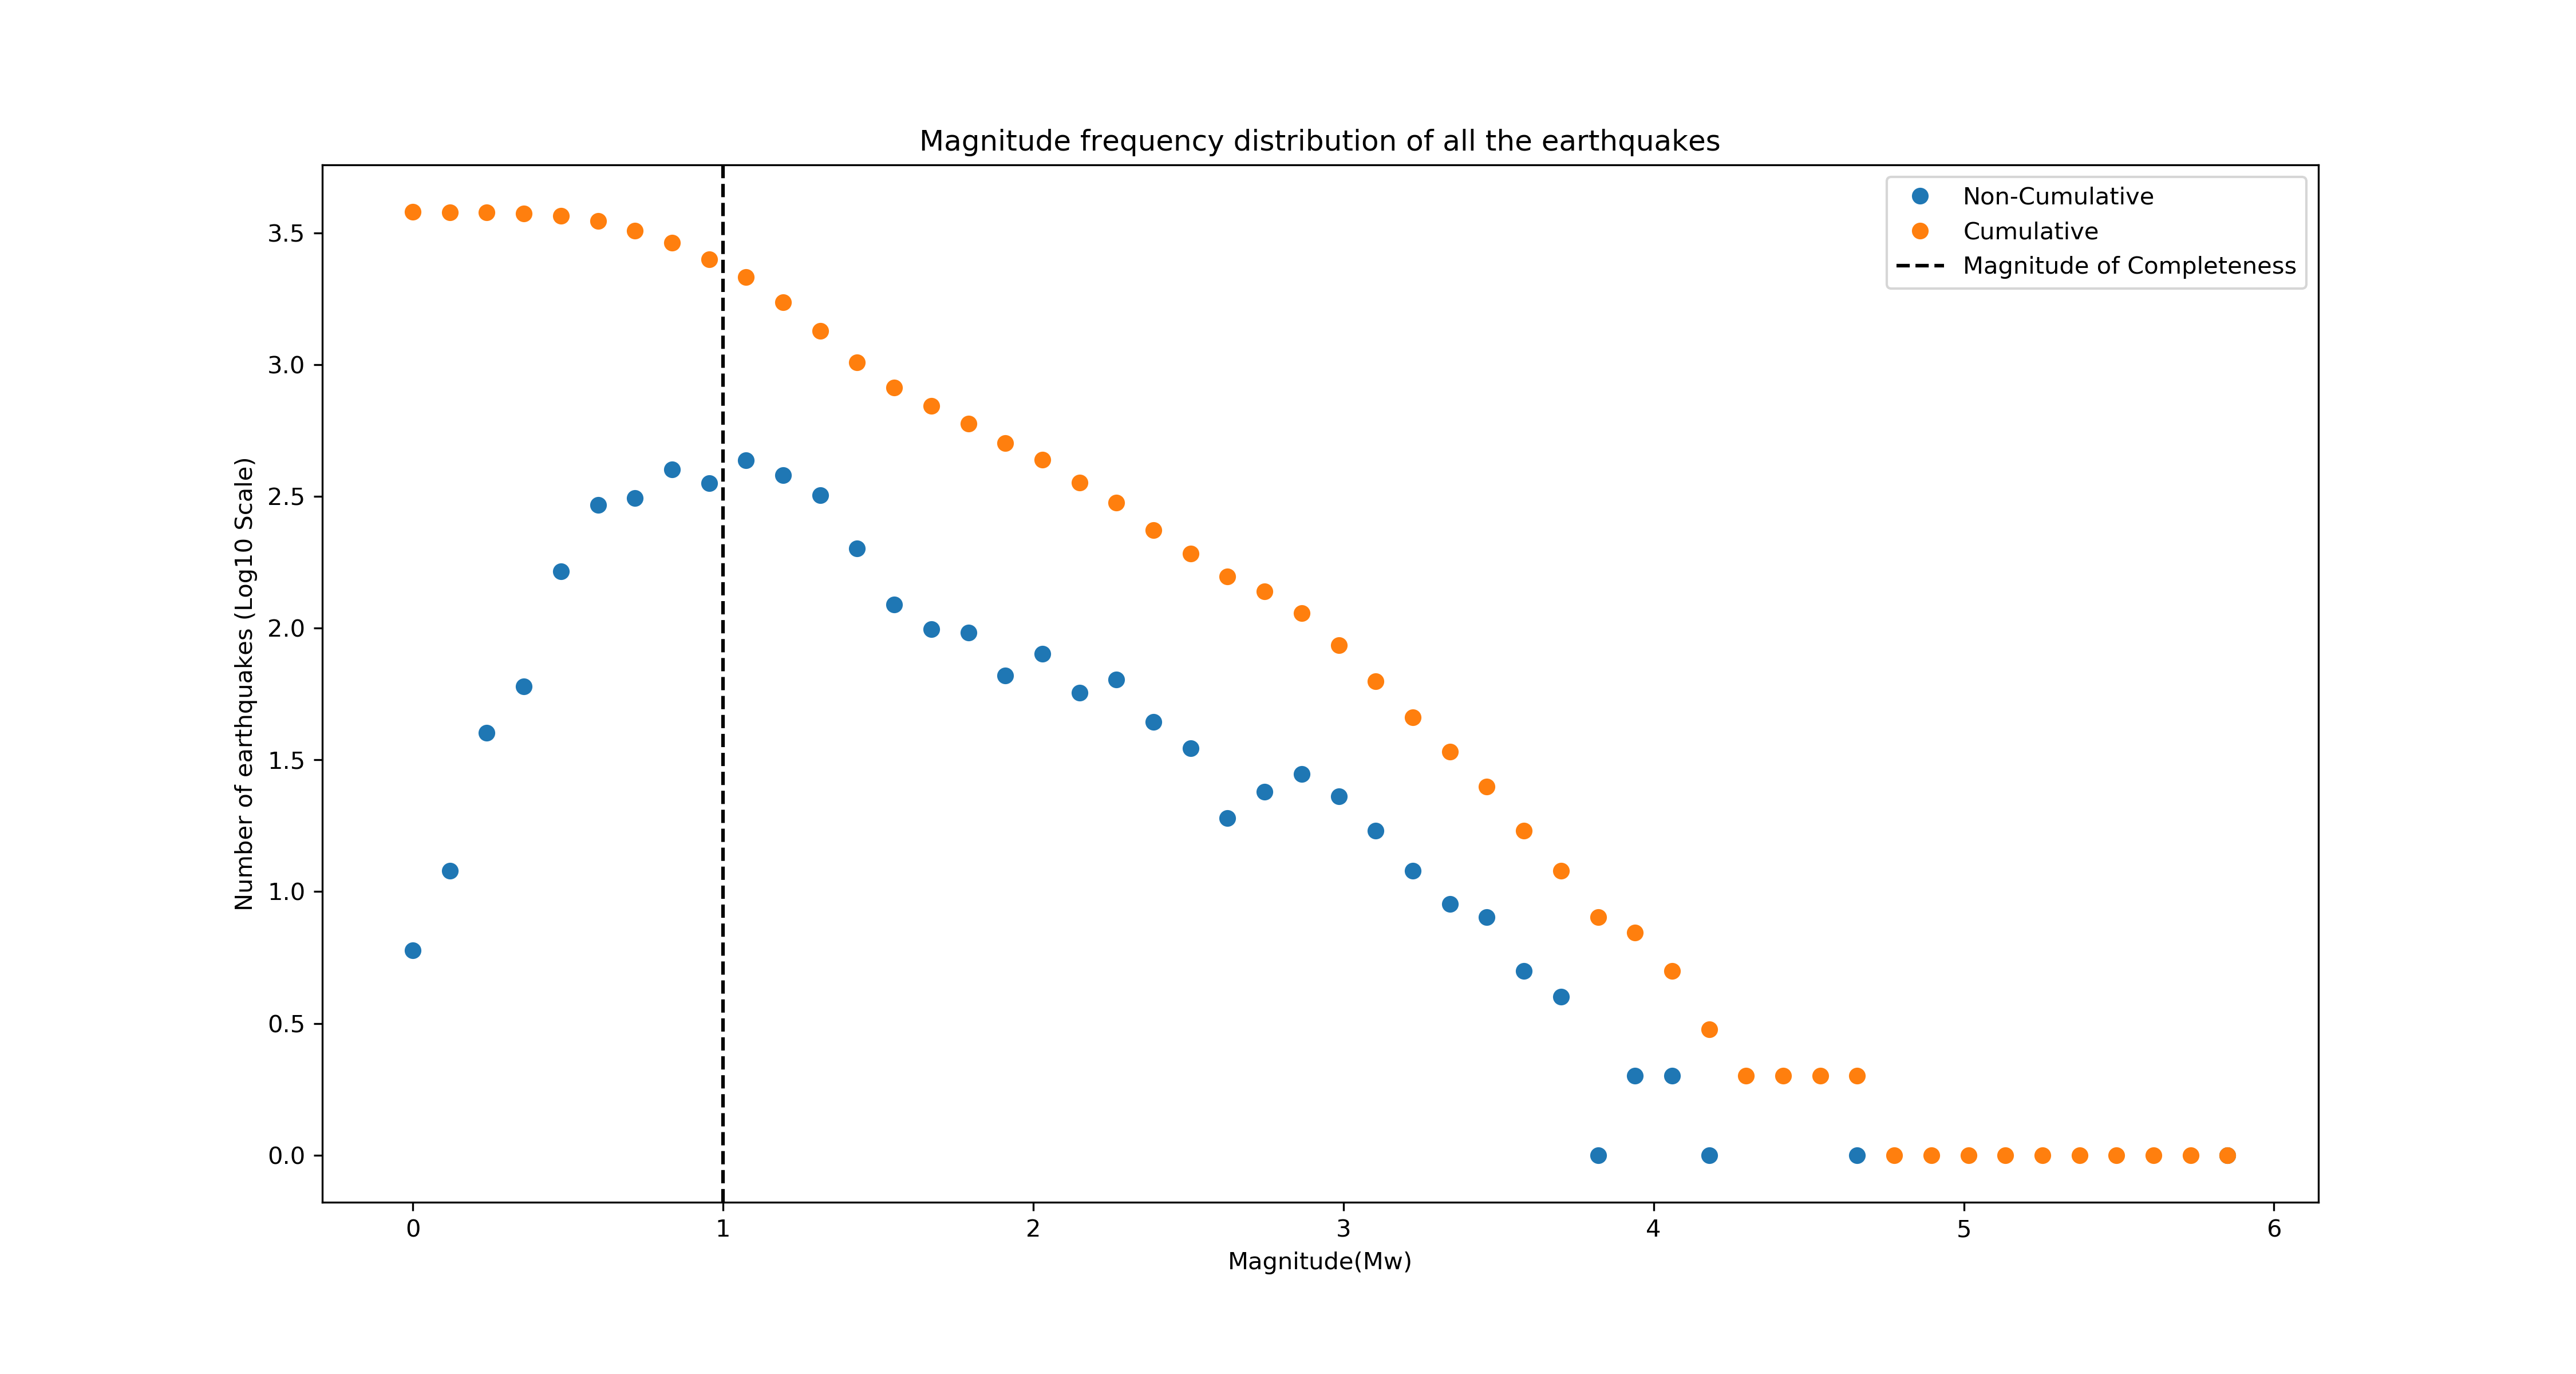
\includegraphics[width=\textwidth]{images/mfd_complete} 
    \end{figure}
\end{frame}

% RESULTS PLOT
\section{Long Fault Zone}
\begin{frame}
    \frametitle{Simulated Results: Fault Zone Depth throughout the Domain}
    \begin{figure}
        \begin{subfigure}[b]{0.5\textwidth}
            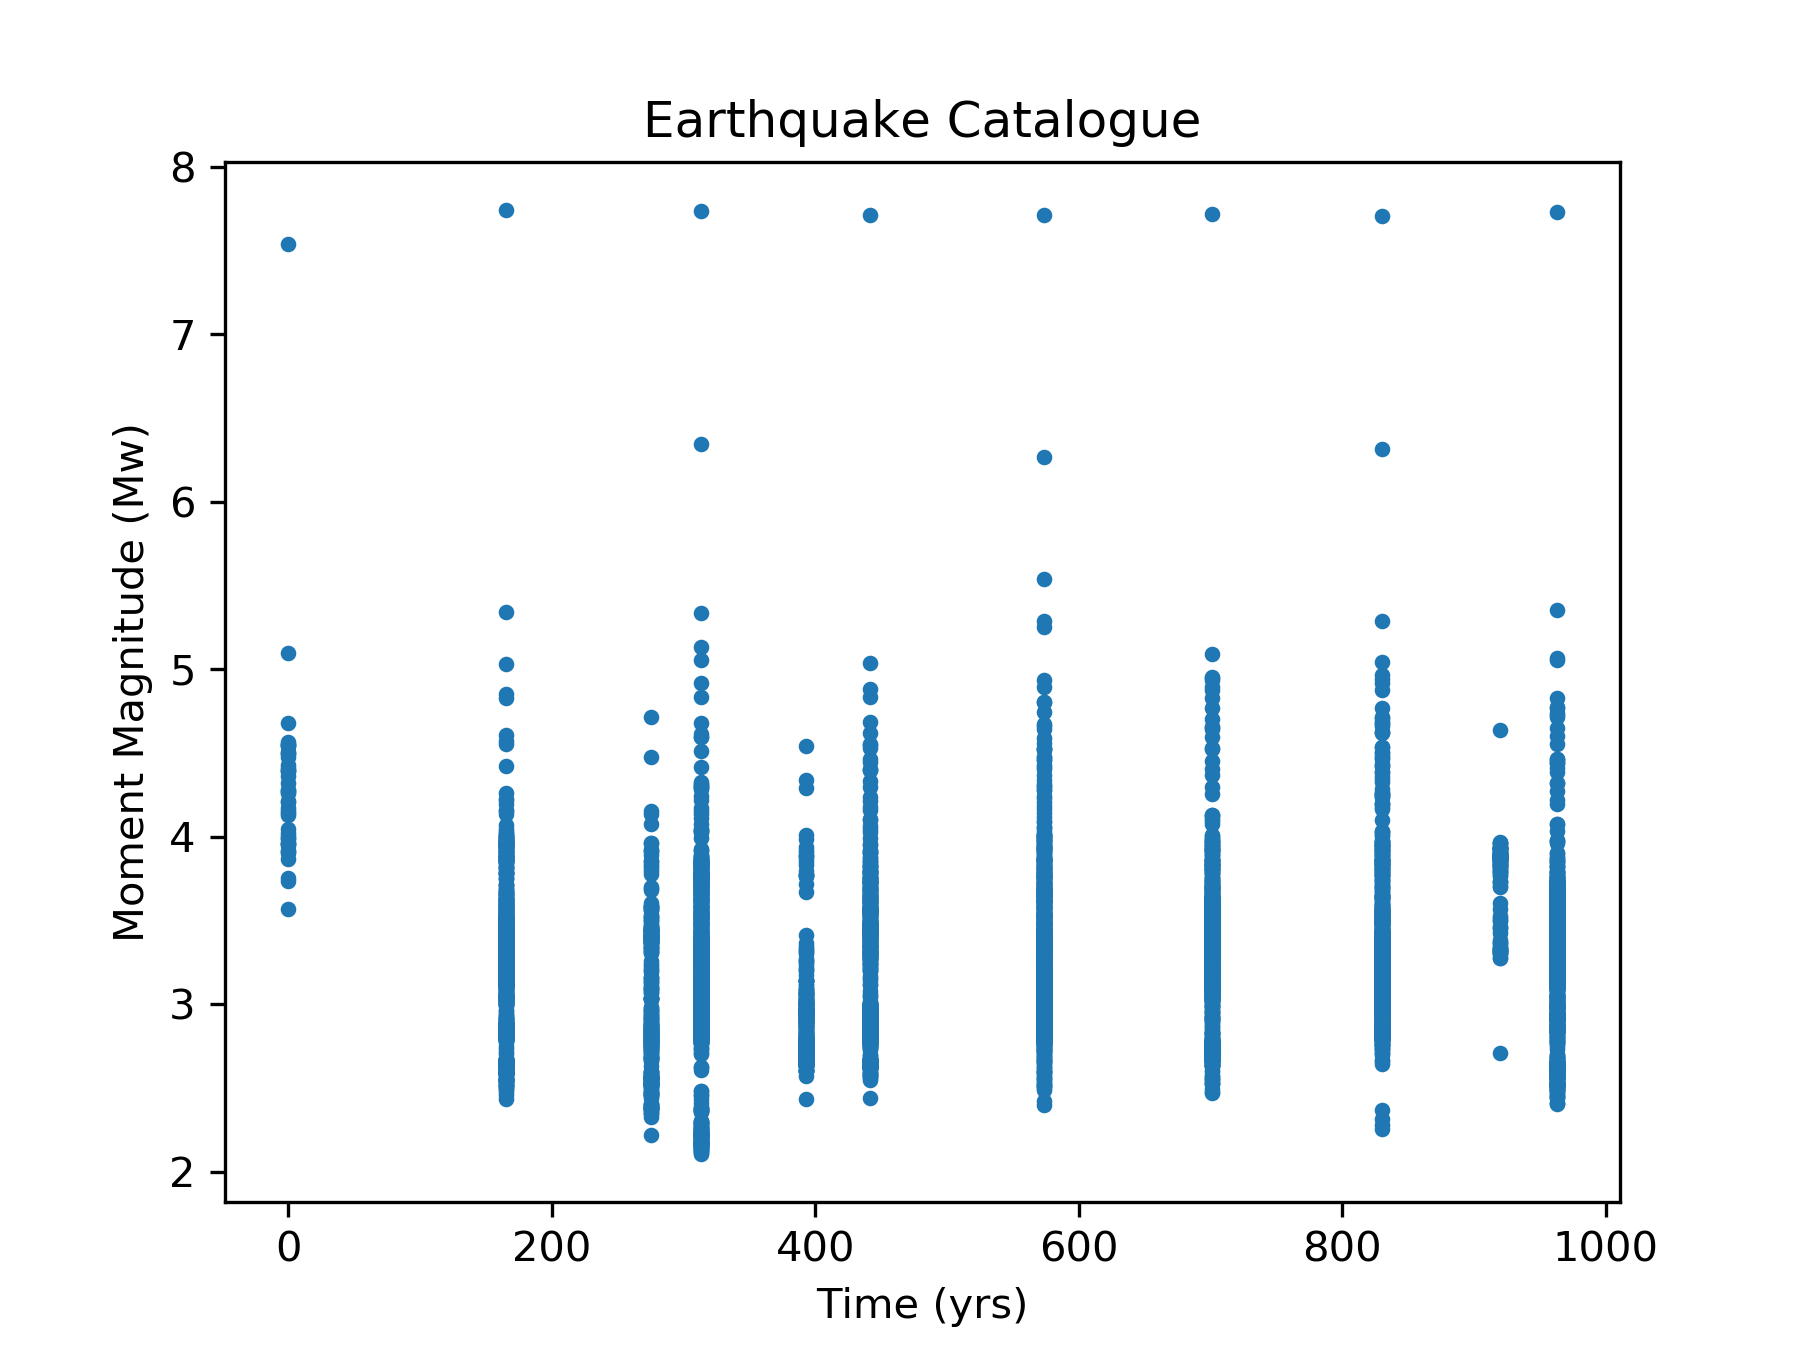
\includegraphics[width=\textwidth]{images/resultlongFZ/catalogue} 
        \end{subfigure}%
        \begin{subfigure}[b]{0.5\textwidth}
            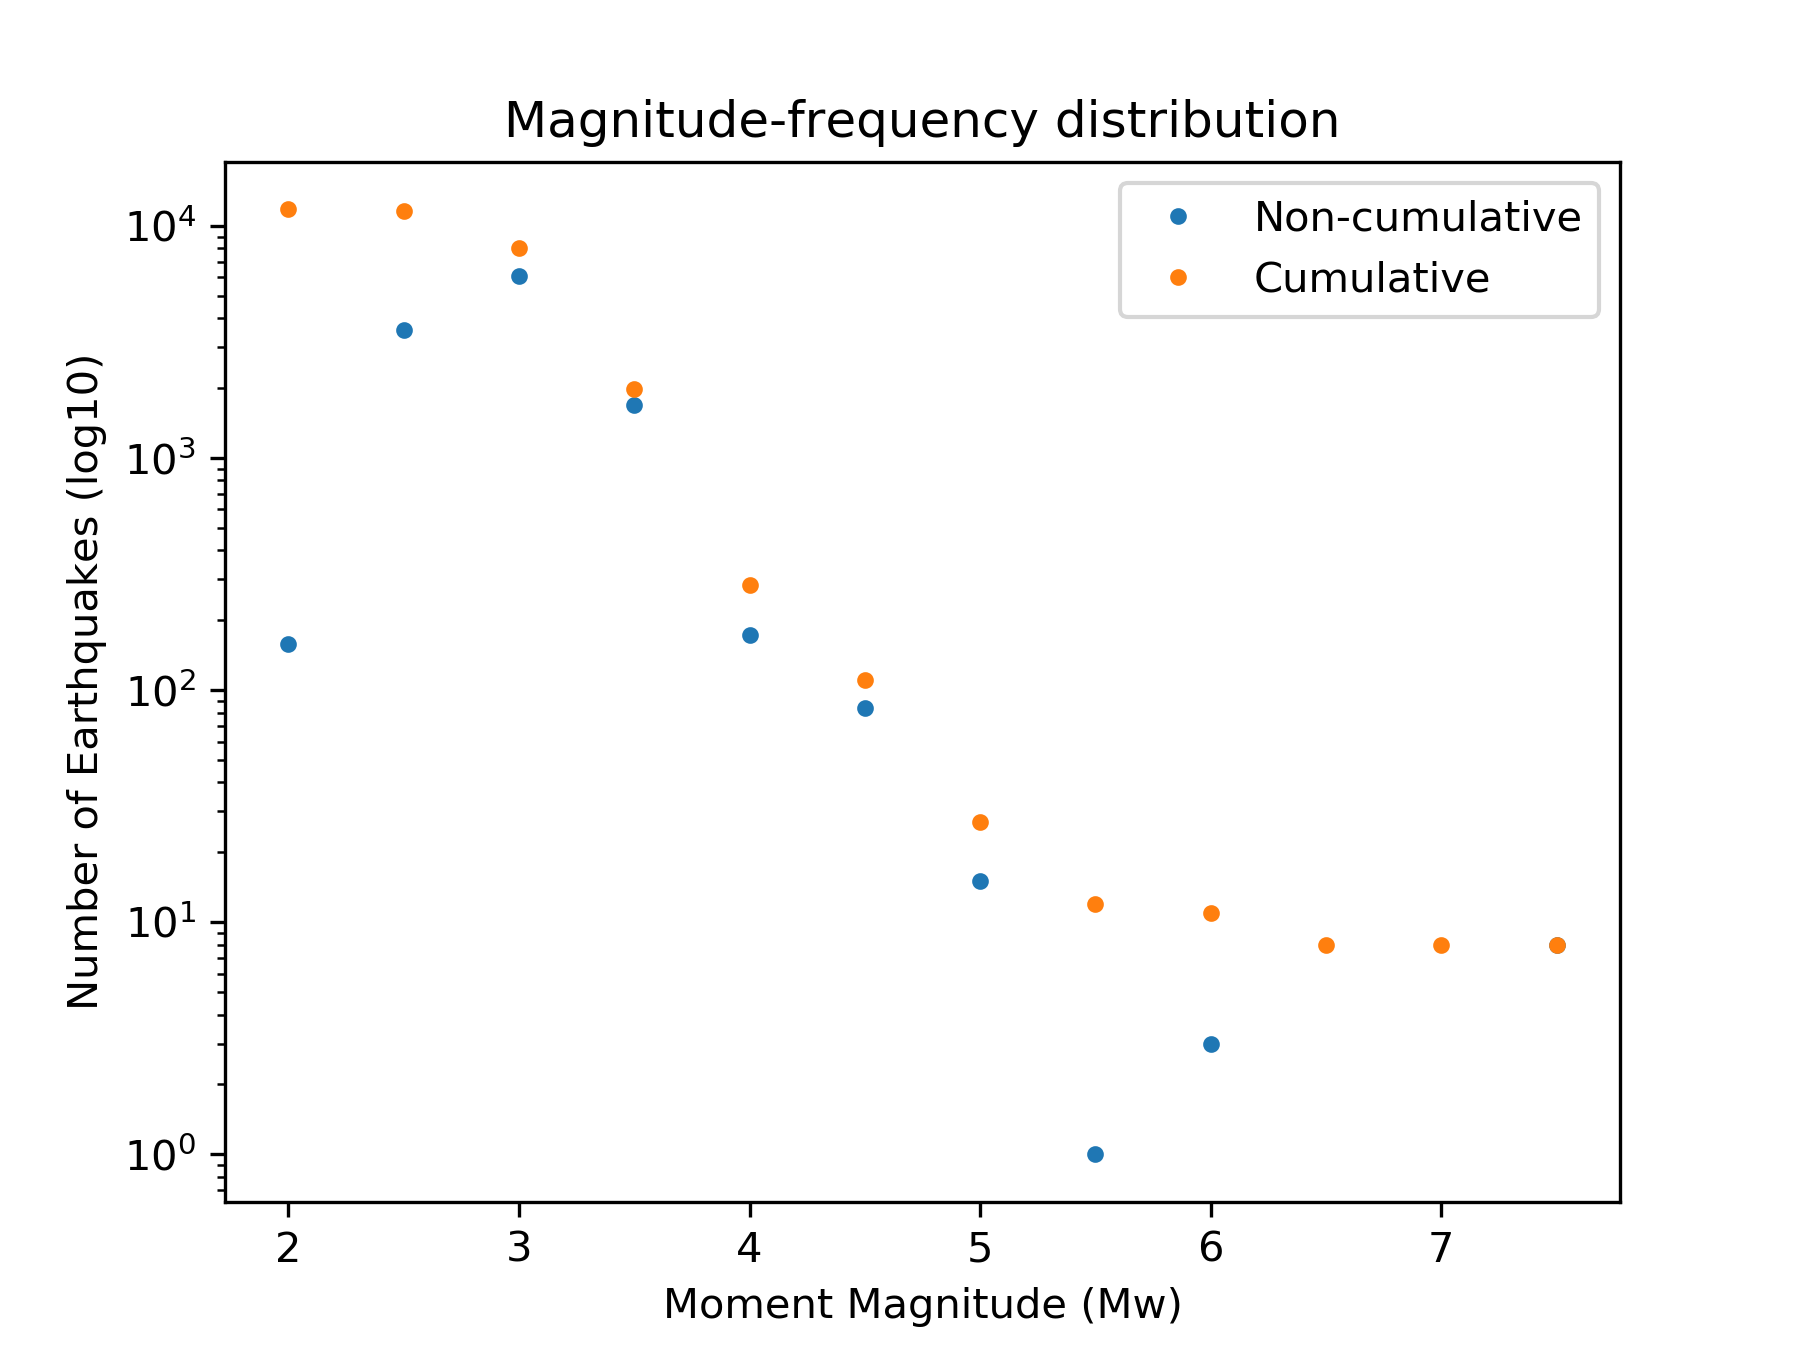
\includegraphics[width=\textwidth]{images/resultlongFZ/mfd}
        \end{subfigure}%
    \end{figure}

\end{frame}

% RESULTS PLOT
\section{Fault Zone depth 8km}
\begin{frame}
    \frametitle{Simulated Results: Fault Zone Depth 8km}
    \begin{figure}
        \begin{subfigure}[b]{0.5\textwidth}
            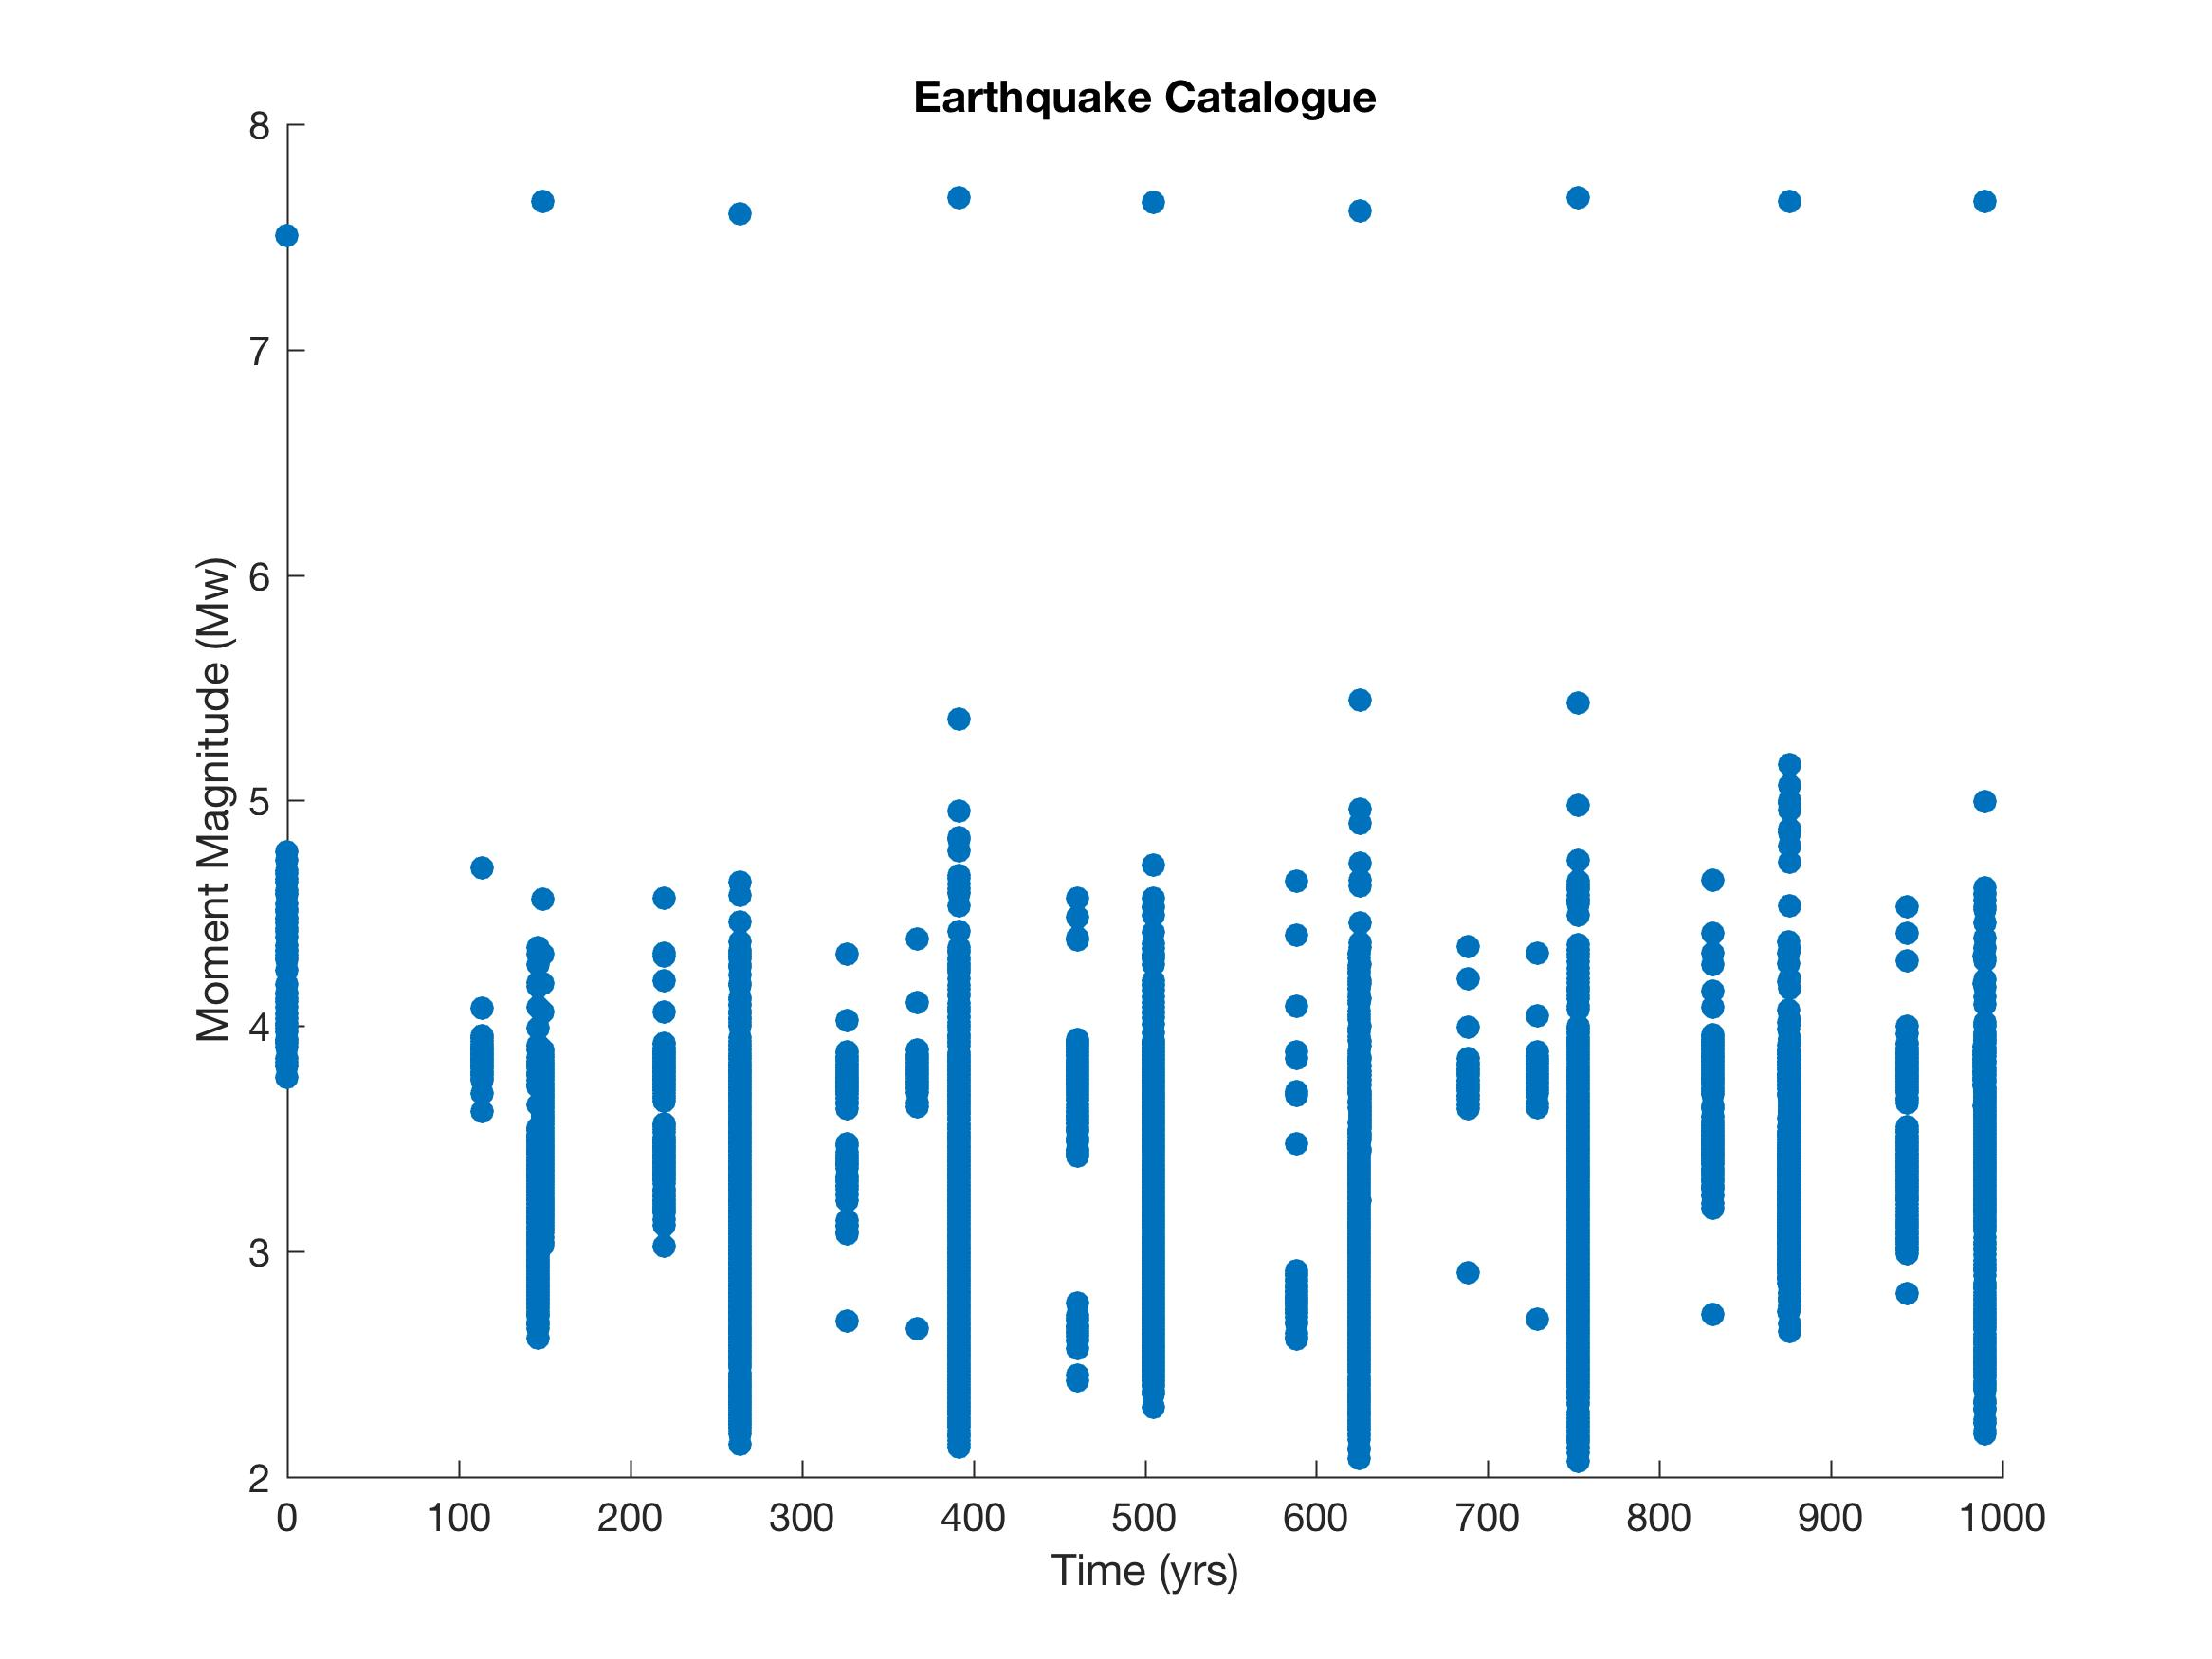
\includegraphics[width=\textwidth]{images/result8km/catalogue} 
        \end{subfigure}%
        \begin{subfigure}[b]{0.5\textwidth}
            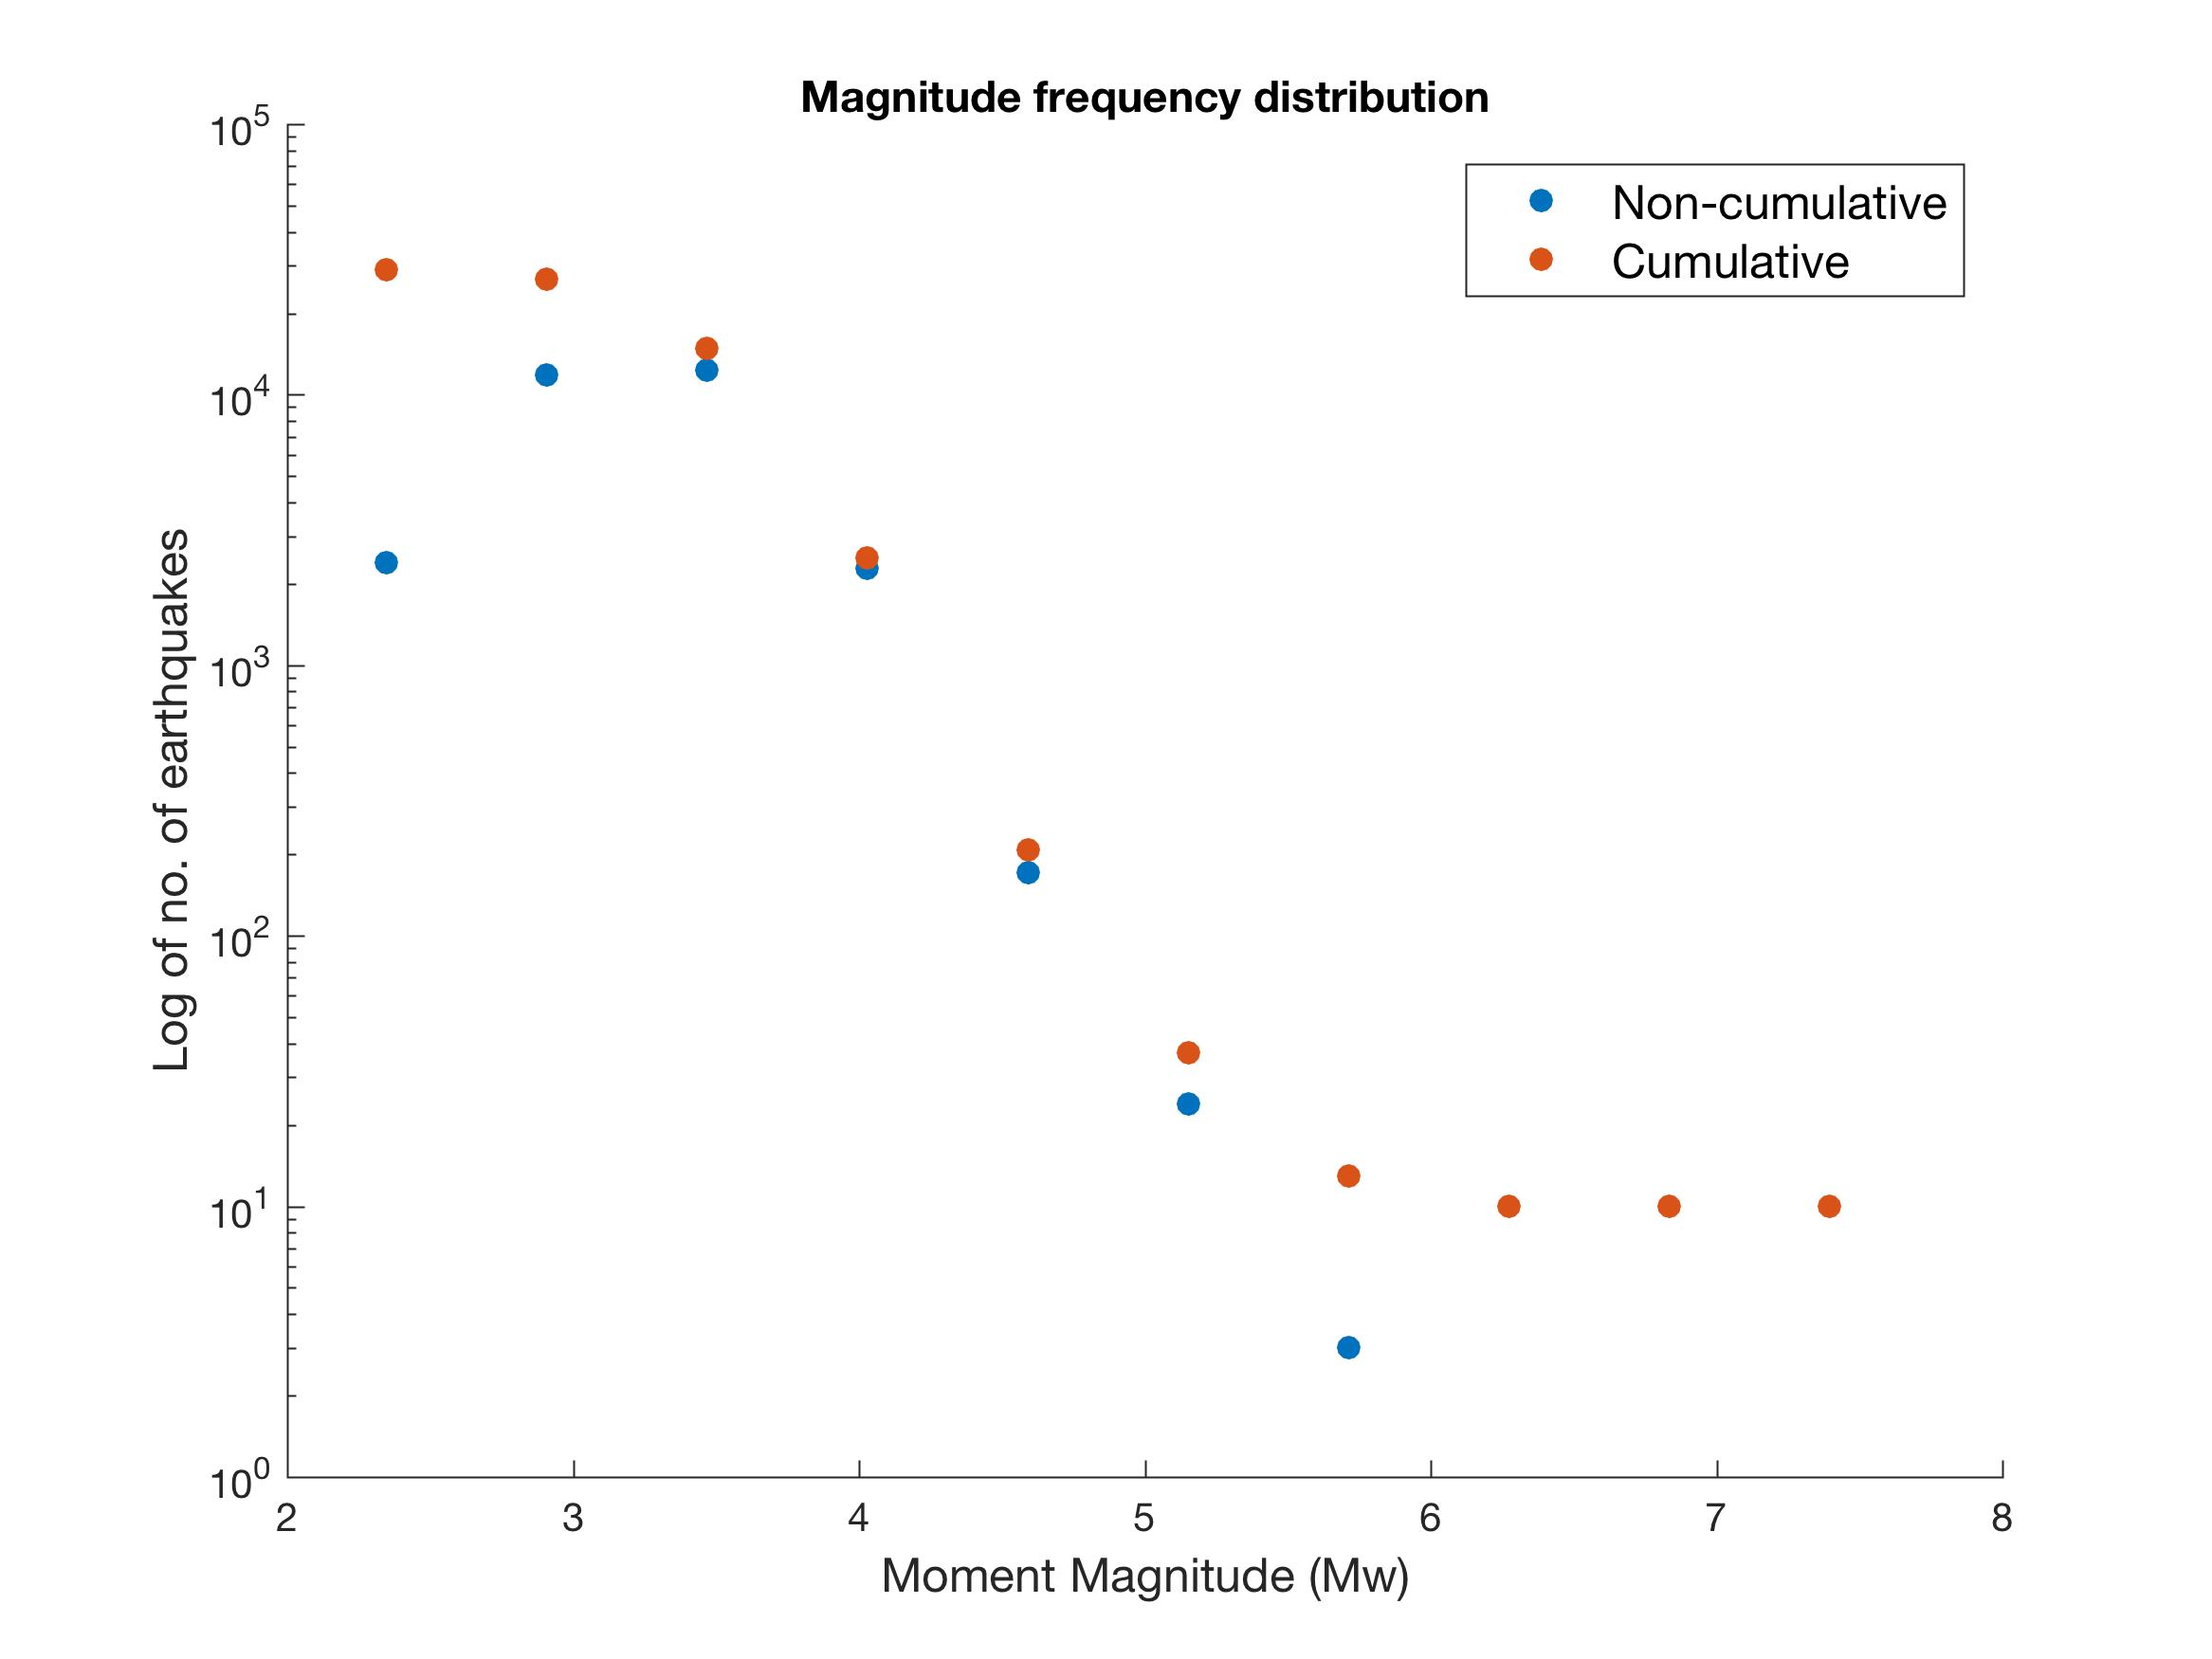
\includegraphics[width=\textwidth]{images/result8km/mfd}
        \end{subfigure}%
    \end{figure}
\end{frame}

% RESULTS PLOT
\section{Fault Zone depth 12km}
\begin{frame}
    \frametitle{Simulated Results: Fault Zone Depth 12km}
    \begin{figure}
        \begin{subfigure}[b]{0.5\textwidth}
            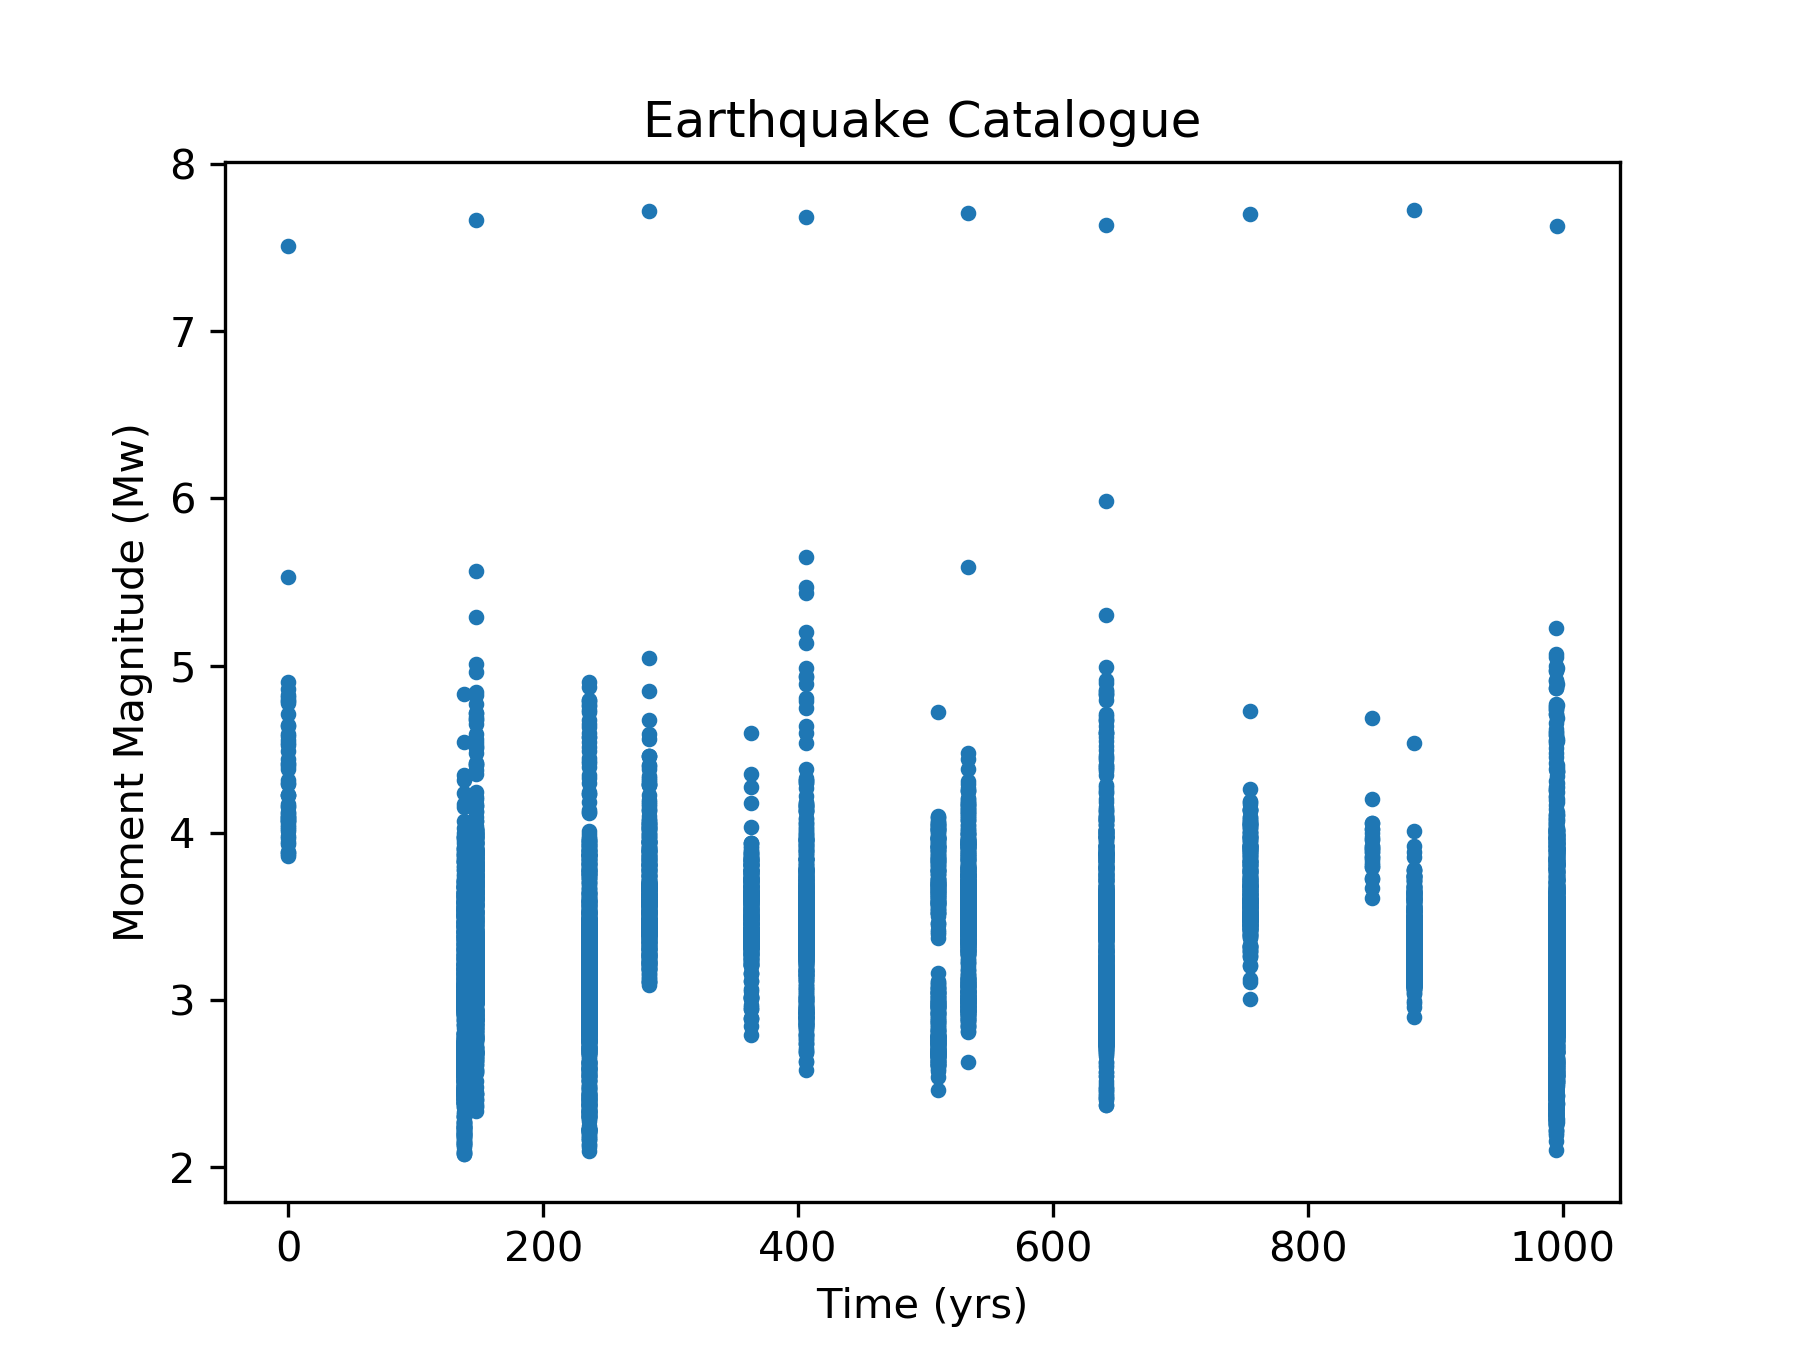
\includegraphics[width=\textwidth]{images/result12km/catalogue} 
        \end{subfigure}%
        \begin{subfigure}[b]{0.5\textwidth}
            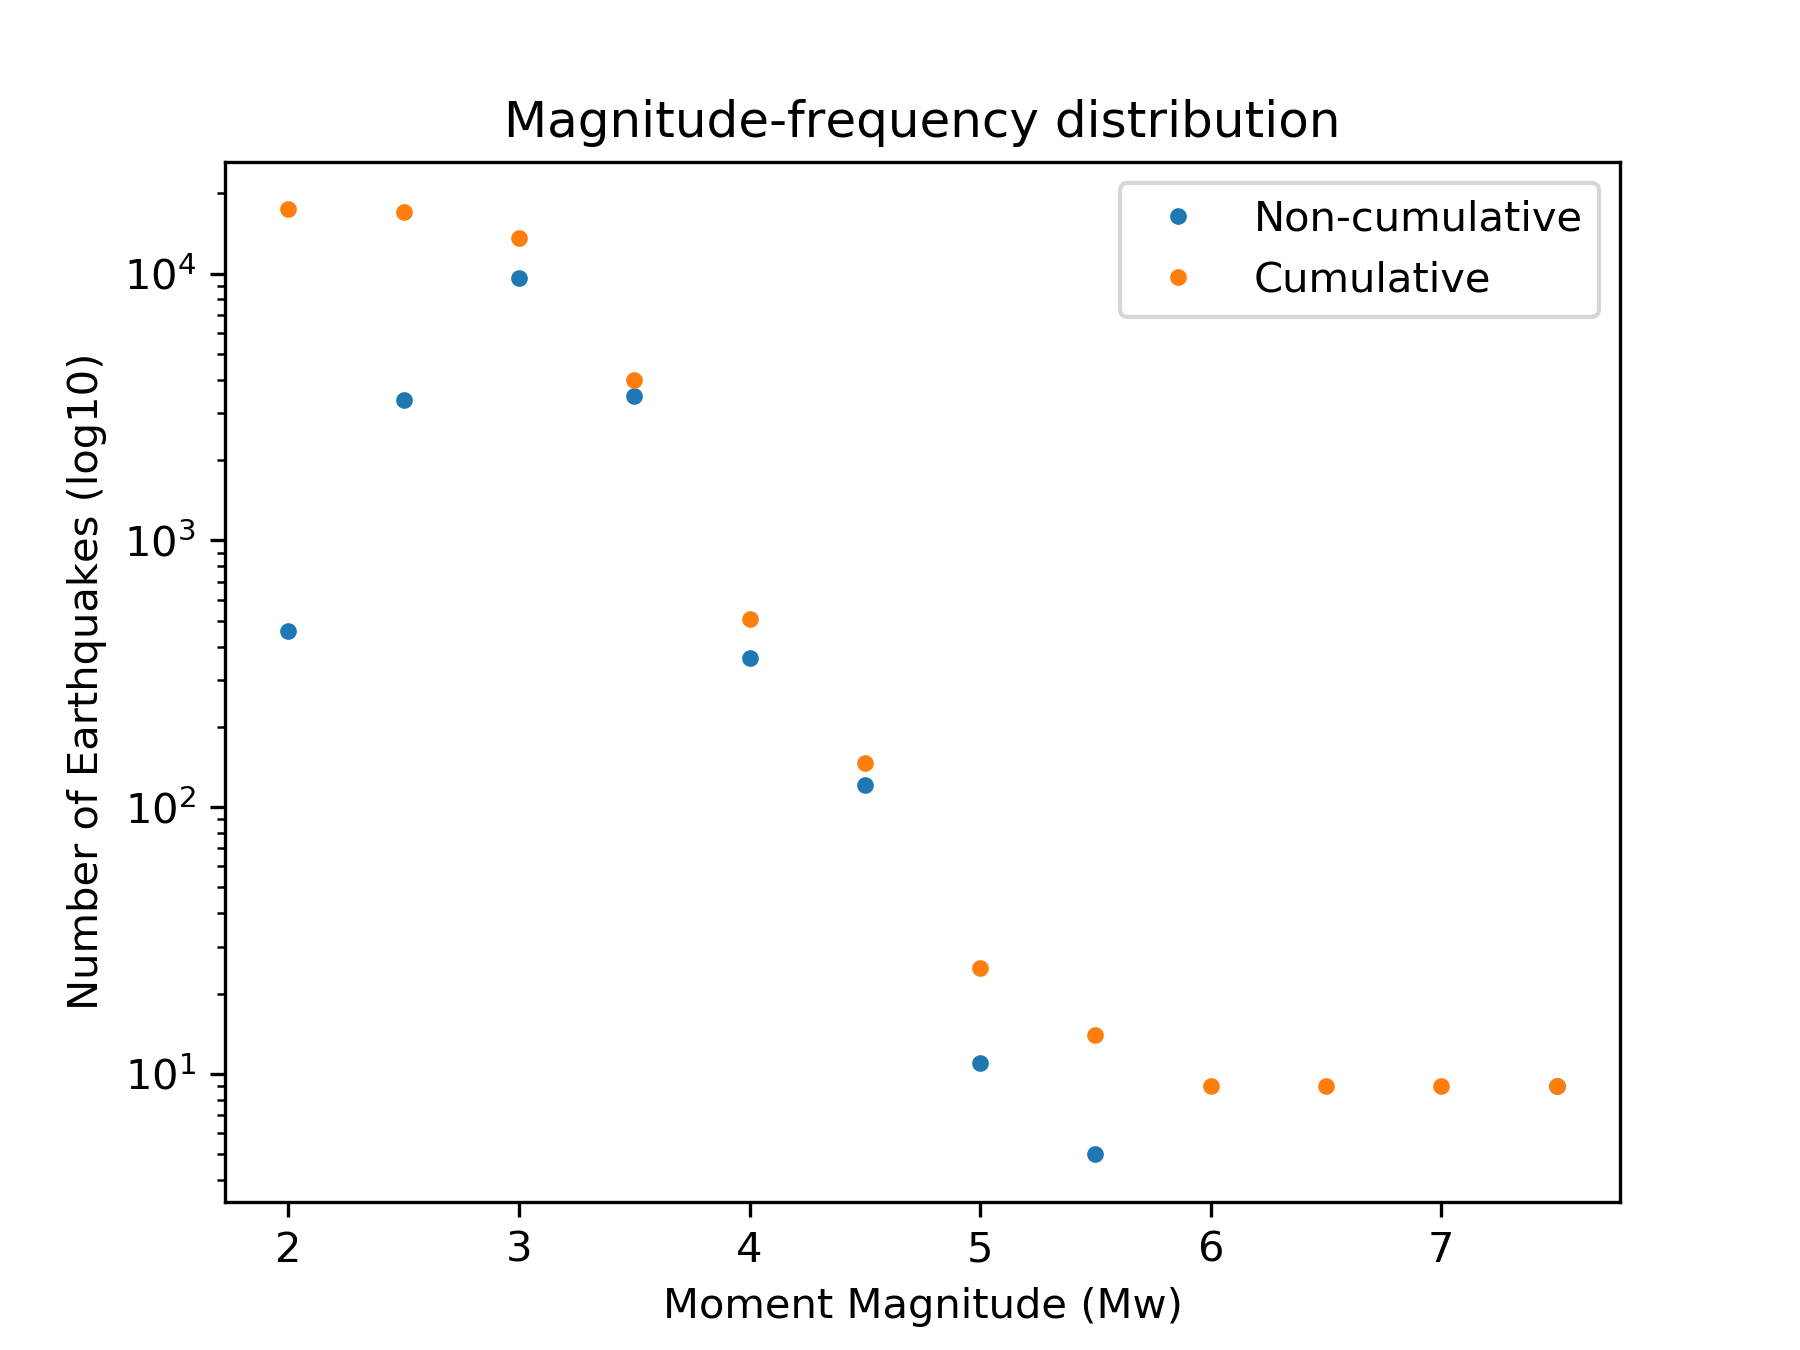
\includegraphics[width=\textwidth]{images/result12km/mfd}
        \end{subfigure}%
    \end{figure}

\end{frame}

% RESULTS PLOT
\section{Stress Drop}
\begin{frame}
    \frametitle{Simulated Results: Stress Drop for Larger Earthquakes}
    \begin{figure}
        \begin{subfigure}[b]{0.5\textwidth}
            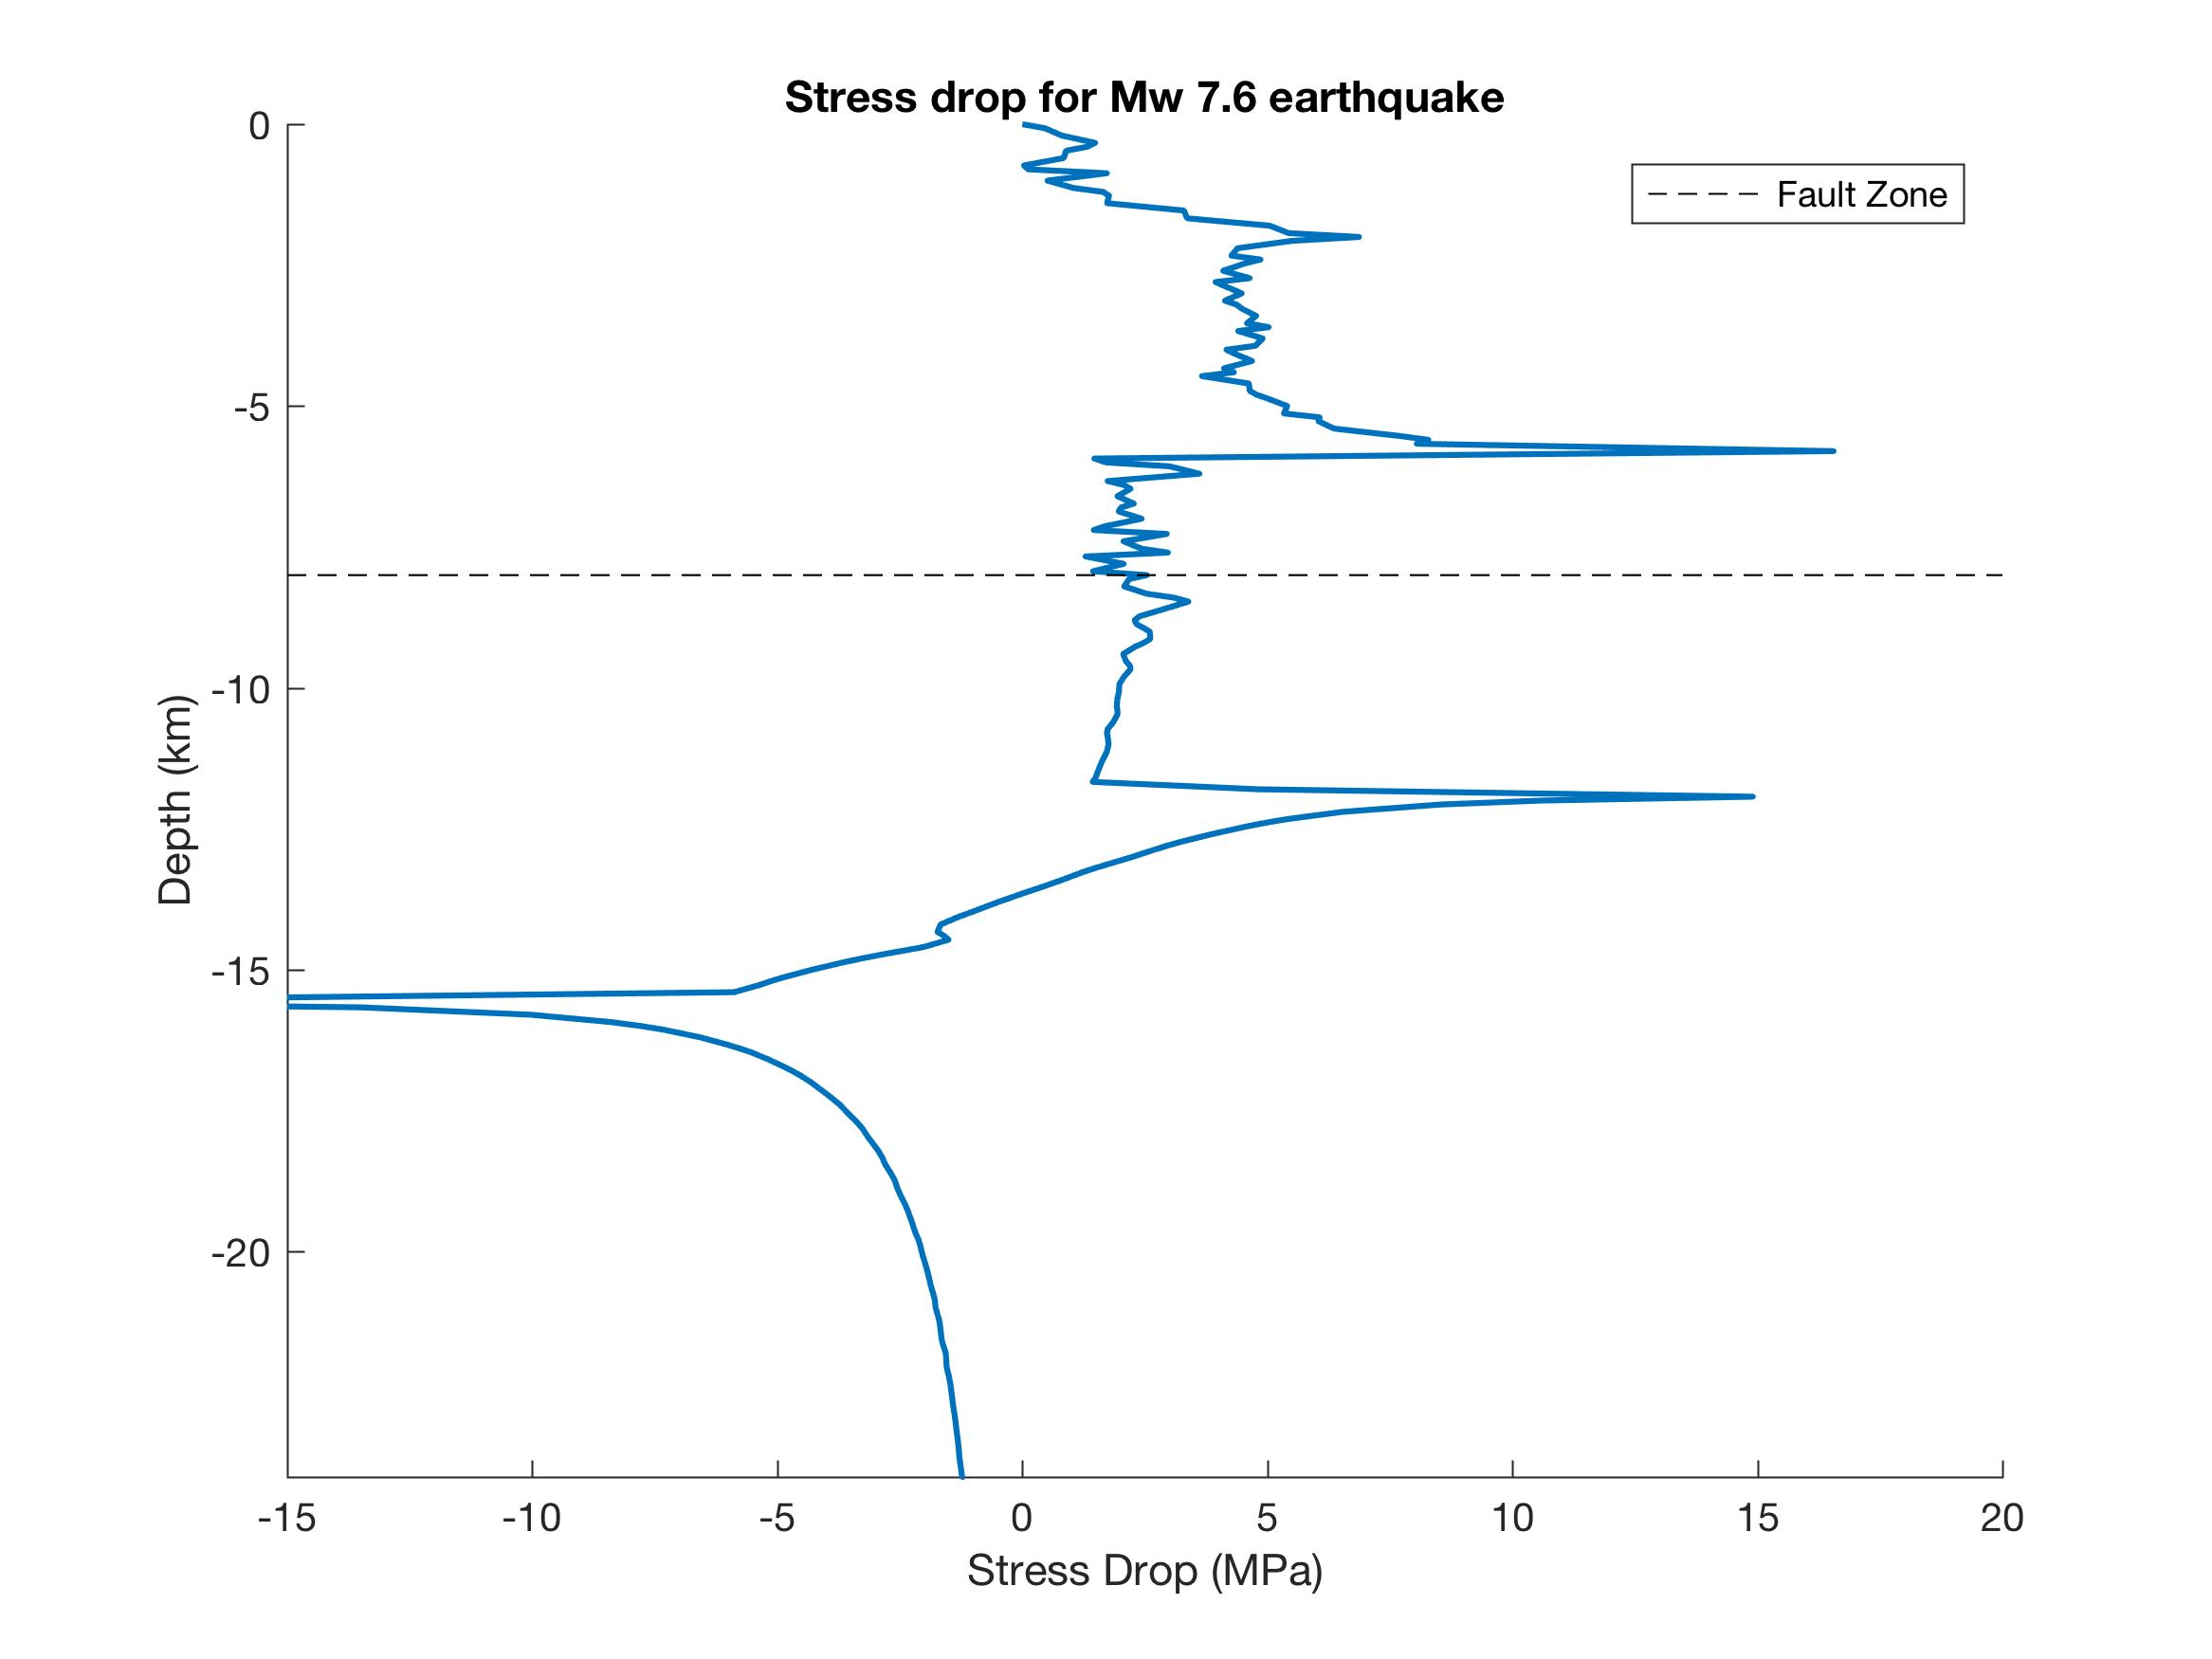
\includegraphics[width=\textwidth]{images/result8km/stress_drop_7} 
        \end{subfigure}%
        \begin{subfigure}[b]{0.5\textwidth}
            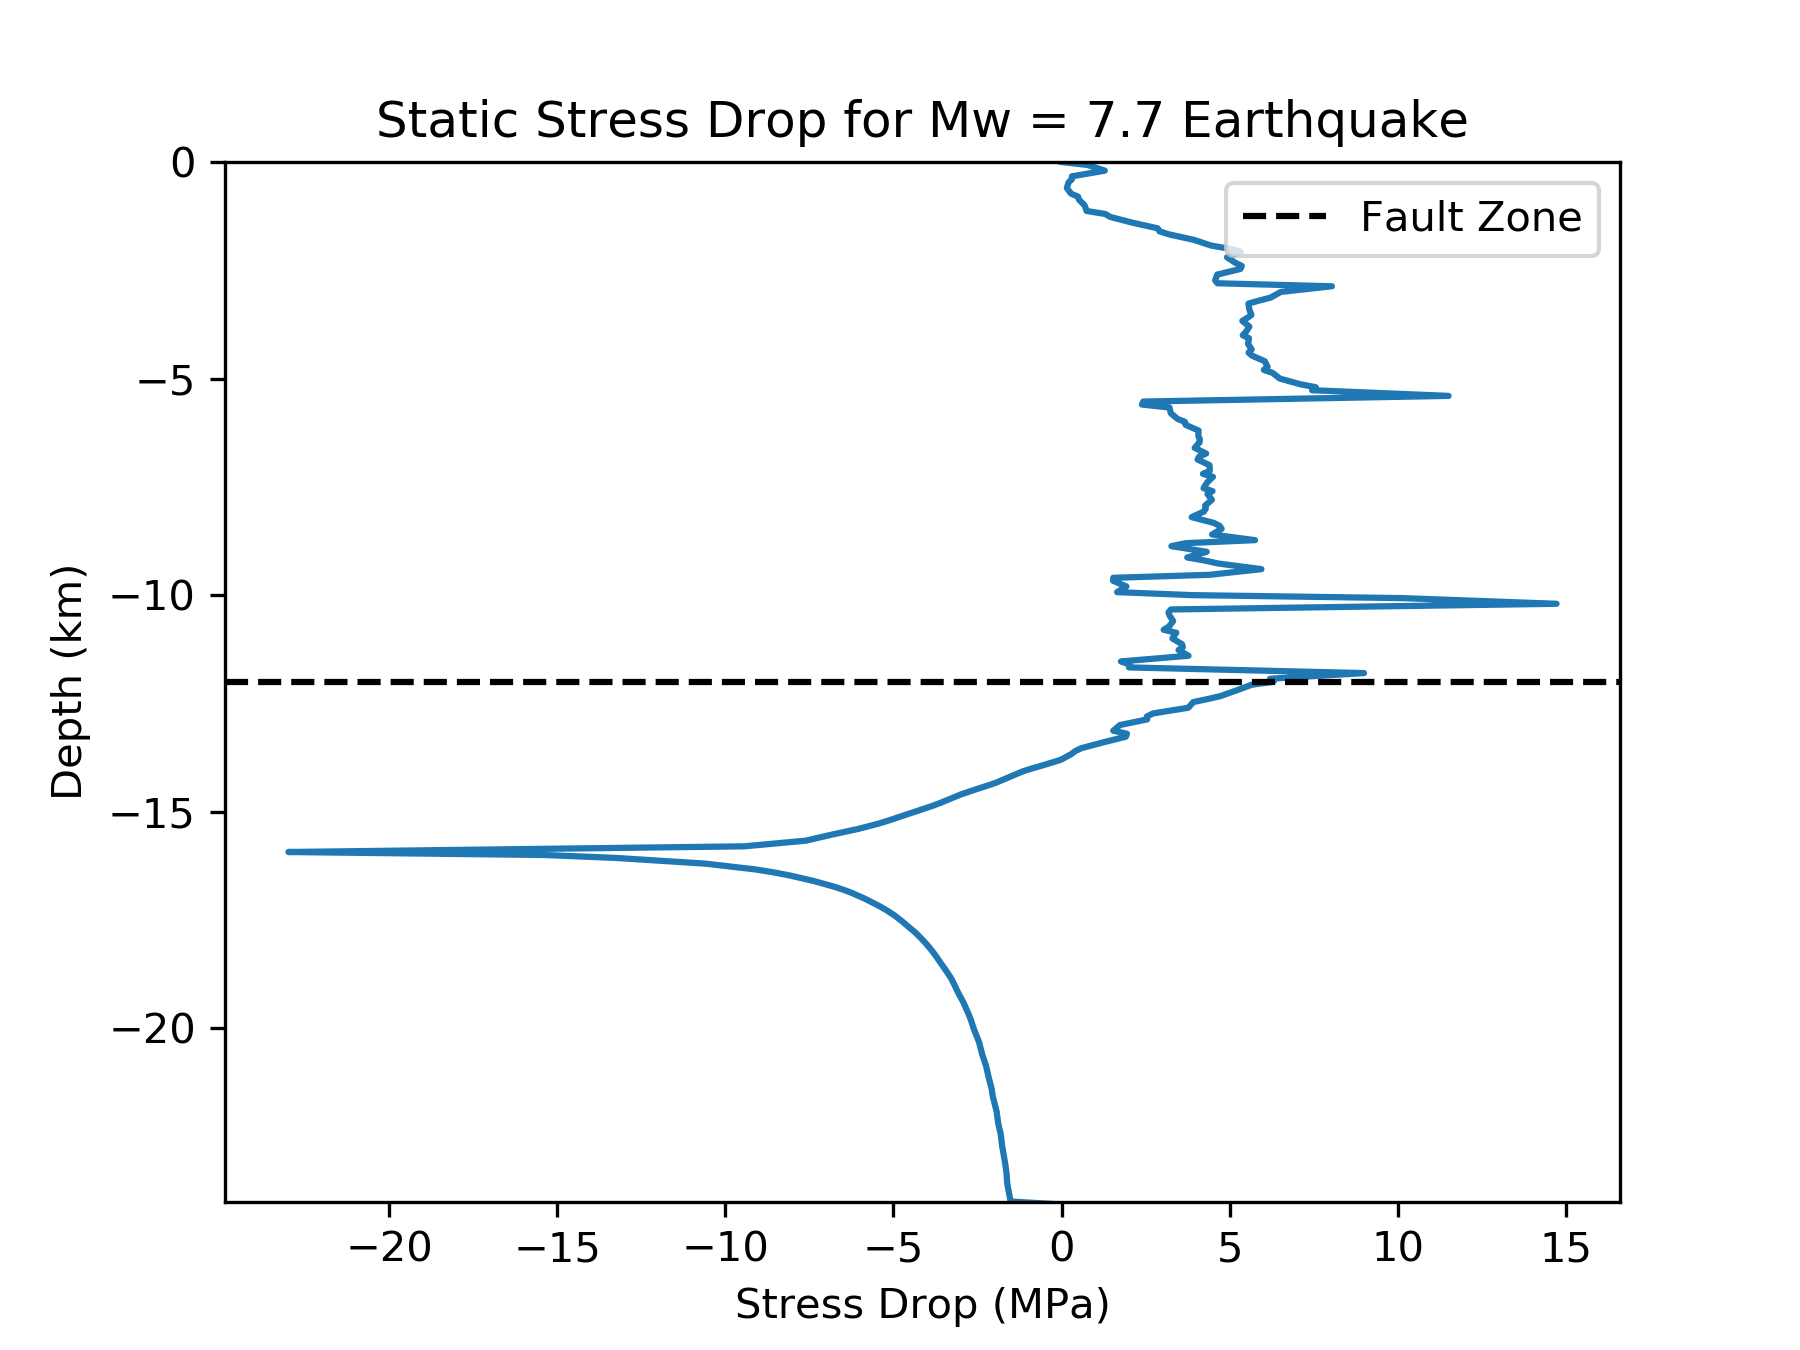
\includegraphics[width=\textwidth]{images/result12km/stress_drop_7}
        \end{subfigure}%
    \end{figure}
\end{frame}

\begin{frame}
    \frametitle{Simulated Results: Stress Drop for Larger Earthquakes}
    \begin{figure}
            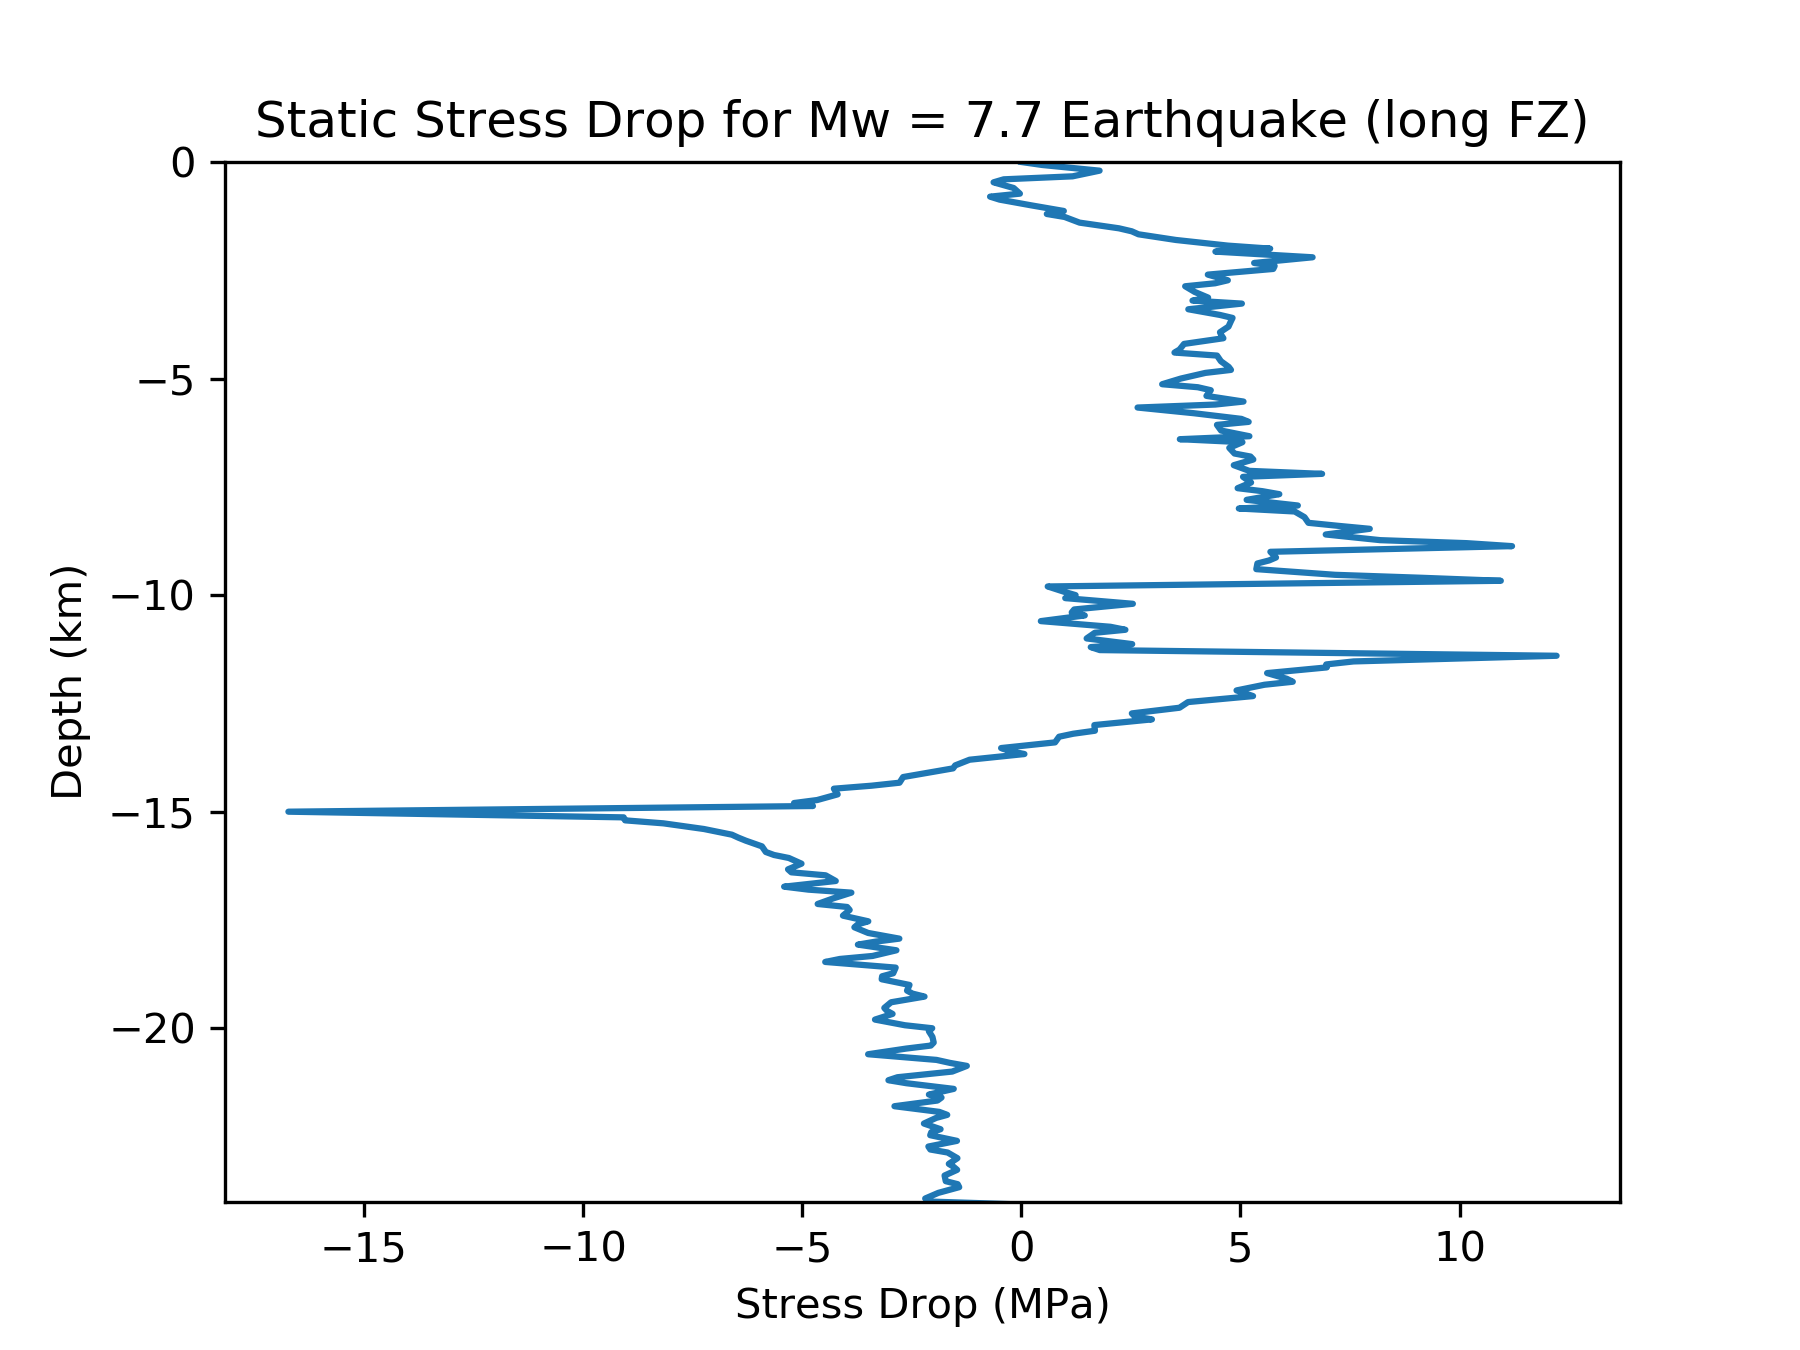
\includegraphics[width=0.5\textwidth]{images/resultlongFZ/stress_drop_7} 
    \end{figure}
\end{frame}

% CONCLUSIONS
\section{Conclusions}
\begin{frame}
    \frametitle{Conclusions}
    \begin{itemize}
        \item The presence of fault zone promotes stress heterogeneity.
        \item This stress heterogeneity gives rise to a power law distribution of earthquakes.
        \item The distribution is more similar to characteristic type earthquake distribution.
        \item Earthquake cycle simulations with dynamic treatment of inertial effects gives a more realistic view of earthquake distribution in the presence of a material heterogeneity.
        \end{itemize}
\end{frame}

% FUTURE WORK
\section{Future Work}
\begin{frame}
    \frametitle{Future Work}
    \begin{itemize}
        \item Implement parallel programming in the code.
        \item A parameter study with a narrower fault zone (400m). Velocity contrast: 20\%, 40\%, 60\%, 80\%. Fault Zone Depth: 5km, 7.5km, 10km, 12.5km, 15km.
        \item Increase cumulative damage after each earthquake cycle.
        \item Write paper and qualifying exam proposal.
    \end{itemize}
\end{frame}

% ENDING SLIDE
\begin{frame}
    \Huge{\centerline{That's All Folks!!}}
\end{frame}
\end{document} 
%%%%%%%%%%%%%%%%
